%%%%%%%%%%%%%%%%%%%%%%%%%%%%%%%%%%%%%%%%%%%%%%%%%%%
%
%  New template code for TAMU Theses and Dissertations starting Spring 2021.  
%
%
%  Author: Thesis Office
%  
%  Last Updated: 1/13/2021
%
%%%%%%%%%%%%%%%%%%%%%%%%%%%%%%%%%%%%%%%%%%%%%%%%%%%

%%%%%%%%%%%%%%%%%%%%%%%%%%%%%%%%%%%%%%%%%%%%%%%%%%%%%%%%%%%%%%%%%%%%%%
%%                           SECTION I
%%%%%%%%%%%%%%%%%%%%%%%%%%%%%%%%%%%%%%%%%%%%%%%%%%%%%%%%%%%%%%%%%%%%%


\pagestyle{plain} % No headers, just page numbers
\pagenumbering{arabic} % Arabic numerals
\setcounter{page}{1}


\chapter{\uppercase {Introduction}}
\label{cha:Introduction}
This dissertation intends to introduce information quality research into the electricity market monitoring industry- a regulatory component of the North American Bulk Electric System (BES) \cite{ferc1} and their corresponding electric markets. Often touted as the "world's largest machine" \cite{stenvignils} by electrical industry staff, the BES has become an important dependency in the lives of virtually every resident of the United States, Canada, and (a portion of) Mexico.

To illustrate the opportunity that superimposing information quality research onto the market monitoring domain poses, this chapter shall introduce the concepts of the BES, electric markets, and Market Monitoring, and provide detail as to how applying information quality concepts to Market Monitoring will help serve a previously unsolved problem within the industry.

\section{The North American Bulk Electric System}

The BES \footnote{The North American Electric Reliability Corporation (NERC) serves as the Electric Reliability Operator (ERO) for the BES. In their Glossary of Terms (see References section), the BES refers to all high-voltage transmission lines and substations, generation resources, and all other equipment used in both inter/intra-state transmission of electric capacity.}
is a highly integrated system that facilitates transmission of electric power (generalized as “energy”) from generation to energy consumption (generalized as a “load”) in a real-time and balanced \footnote{The term “balancing” refers to the need to only generate power as it is needed for consumption- subject to system capacity and economic constraints.}
manner. With few (relatively recent) exceptions \footnote{Storage resources are a developing technology that can store energy for deployment during reliability emergencies or intervals of energy scarcity.}
, energy is not stored in the system; it is generated (in response to a demand forecast) and then immediately transmitted and consumed by various loads. Figure \ref{fig:BES_1} shows a conceptual configuration of some of the components \footnote{An important distinction to note is between the \textit{utility} and \textit{retail} sectors shown in Figure \ref{fig:BES_1}. While referred to by several names (i.e. wholesale), utility generation and transmission refers to bulk energy (on the scale of MW) that is transmitted on the BES. The retails sector involves distribution of energy to residences and low consumption (on the scale of kW) commercial enterprises. This research focuses on wholesale energy markets, and thus is concerned with the bulk power generation and transmission domains.}
involved in the operation of the BES. \cite{devasia}

The BES must be precisely managed, at all times, to balance power across the system and to serve load. Deviations can cause significant damage to BES infrastructure, as were seen during the February 2021 Winter Storm in Texas' electric grid \cite{balancing1}.
No one entity manages the entire BES. Instead, this job is shared across geographic locales. This paper focuses specifically on support for organized markets, which pool resources managed by a Regional Transmission Organization (RTO) or an Independent System Operator (ISO). These entities serve multiple roles; their primary role is to function as a grid operator. These organizations commit and dispatch electric generation (a coal plant or a wind farm, for example) based on the principle of security-constrained economic dispatch (SCED)
\footnote{Economic dispatch ("ED") is a concept that blends economics and the physical reality of the electric grid.}.

These organizations also frequently act as Reliability Coordinators (RC) and Balancing Authorities (BA), monitoring power flows, balancing the grid, and acting to restore system reliability during and after an emergency. One such function provided by BAs includes corrective frequency response. Many lay-persons are likely aware that the US electric grid operates, synchronously, at 60 Hz (or, 60 cycles per second). On such a broad scale, the collection of companies and regulation entities that operate the grid must also ensure minimal deviation from this baseline of 60 Hz. A broader engineering discourse of the electric generation and reliability functions of the BES is outside of the scope of this work.

\begin{figure}
\centering
\fbox{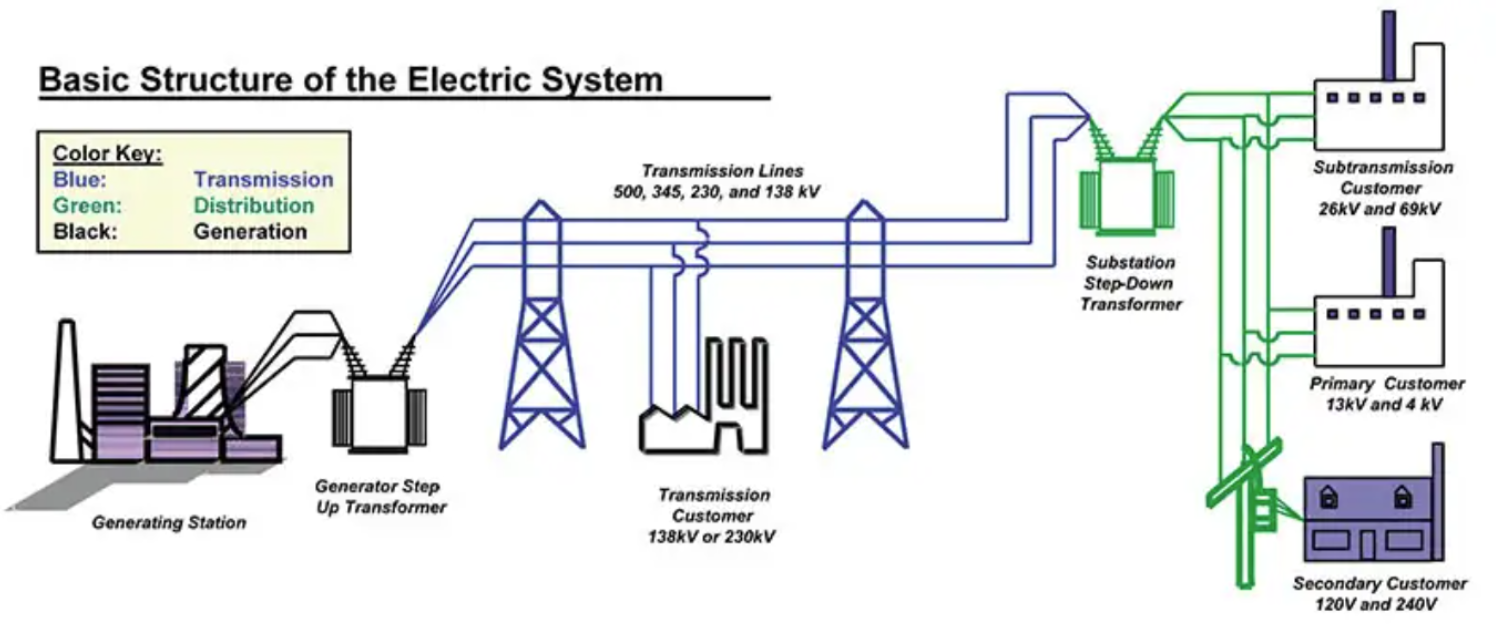
\includegraphics[scale=0.365]{graphic/basic-structure-of-the-bes.png}}
\caption{A conceptual illustration of the Bulk Electric System} 
\label{fig:BES_1}
\end{figure}

It is important to note that serving these various functions to provide electricity generates enormous amounts of data on an hourly basis. This data is widely diverse in terms of sourcing, formatting, usage, sensitivity, and volume. It is the data assets generated by the operation of the BES that serve as the focus of this dissertation, specifically in the data generated by \textit{electricity markets}.
\section{An Introduction to Electricity Markets}

A basic understanding of economics includes the concepts of supply and demand. Supply indicates that a seller has a good (usually a commodity \footnote{Commodities refer to the raw materials that are involved with manufacturing products. For example, crude oil is a commodity that is refined into kerosene, diesel, or gasoline.}
or product). When a consumer wishes to purchase that supply, it is referred to as a demand. The sale of supply results in the formation of a market. As stated above, this paper focuses on organized markets.  A large portion of the BES includes centrally organized electricity markets. Electricity markets are of great importance to all stakeholders involved in the BES; they allow energy to be economically generated for consumers.

\begin{figure}[ht]
\centering
\fbox{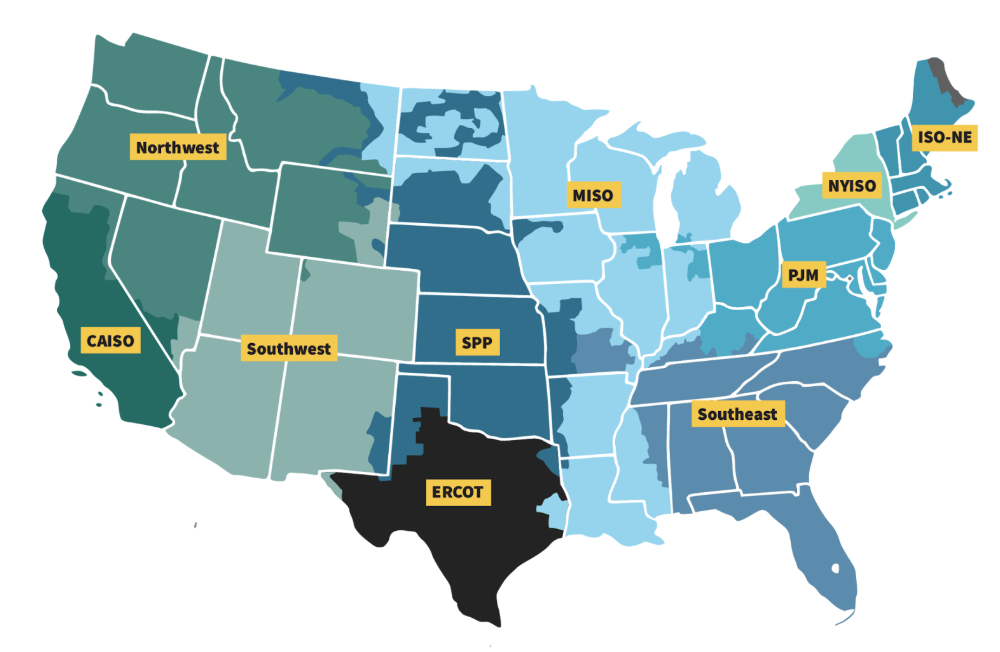
\includegraphics[scale=0.45]{graphic/us-grid-map.png}}
\caption{FERC Jurisdictional Market Territories}
\label{fig:gridmap}
\end{figure}

Figure \ref{fig:gridmap} \cite{ferc2} displays, at a high level, how the US energy grid is divided into different territories. These territories are typically governed by FERC, with the exception of Texas. ERCOT, the electric system operator for Texas, is not within the jurisdiction of FERC. The Public Utility Commission of Texas, instead, has oversight of the ERCOT market territory.

\subsection{Grid Operational Entities}
Electricity markets are operated by a small number of operational entities \footnote{"Grid Operational Entities", as referred to in this chapter, are not limited to the 2 categories listed. They also include Transmission Owners and Operators (TO / TOP), Regional Entities (RE), Balancing Authorities (BA), Reliability Coordinators (RC), and Federal Power Agencies. Oftentimes, an RTO or ISO will also support one or more of these functions (SPP, for example, hosts operational desks for performing reliability coordination).}
within North America. These entities fall under the jurisdiction of FERC, as indicated by Figure \ref{fig:gridmap}. The prominent entities that are impacted by market monitoring include Independent System Operators (ISO) and Regional Transmission Organizations (RTO). These entities are filed as non-profit businesses and typically perform similar functions. FERC Orders 888 and 889 initiated the formalized incorporation of an ISO, while FERC Order 2000 set forth the criteria that differentiates an ISO from an RTO.

\subsubsection{Independent System Operator (ISO)}

ISOs are organizations that manage power generation and transmission across the bulk electric system. They operate in an advisory capacity for generation owners (public and investor owned utilities, as well as independent power producers) and transmission owners and operators to effectively generate and trade power in an energy market. A common, helpful analogy that describes the function of an ISO is an air-traffic controller.

Air-traffic controllers merely monitor and route airplane traffic across the airspace over the United States. They own neither physical airplanes nor airlines, and function only as advisors to ensure safe passage of both private and commercial airplanes. ISOs work in a similar fashion. The ISO over the California energy market territory (CAISO) owns none of the transmission infrastructure across which electric power is shipped. However, CAISO manages the flow of energy across this system, and sends regular dispatch instructions to the generators that inject power into the BES.

\subsubsection{Regional Transmission Organization (RTO)}

According to the \textit{Energy KnowledgeBase} product maintained by Enerdynamics (an educational entity in the energy space), RTOs are categorized by a group of four core characteristics (and an additional seven broad operational functions). %CITATION% goes here...  item number 3 from original bibliography
The following lists identify these characteristics and functions that separate ISOs and RTOs. Although similar in nature; in fact, they are regulated by the same entities and have many of the same requirements under current law. It is important to note, however, that ISOs also operate energy markets and are subject to the same market monitoring requirements as RTOs. \\


\noindent Core characteristics of an RTO include:
\begin{enumerate}
    \item{Independent operation and authority from the market participants that join the RTO}
    \item{Maintain a "regional configuration"}
    \item{Maintain "operational authority for all transmission facilities under RTO control"}
    \item{Maintain short-term reliability of their footprint}
\end{enumerate}


\noindent Operational functions of an RTO include:
\begin{enumerate}
\item{Energy market design and “tariff administration”}
\item{Management of transmission capacity (FTR)}
\item{Management of flow on the transmission system}
\item{Support for ancillary services (AS)}
\item{Management of transmission capacity and capability, including imports and exports of power}
\item{Engineering support for planning the future state of the gid}
\item{Coordination between control boundaries}
\item{Market Monitoring}

\end{enumerate}

\subsection{Types of Markets}

Electricity markets are designed to serve one of several purposes. ISOs typically deploy and operate these different market designs, in concert, as a \textit{marketplace} \cite{ferc2}. Southwest Power Pool's (SPP) Integrated Marketplace is such an example of this. To understand the scope of market monitoring activities, it is important to understand the main energy market designs that exist today. Arguably, there are five main types of electric energy market designs; each design may be deployed with possible variations on their theme (a marketplace that does not operate the function of a capacity market is one such example). Reference Table \ref{tab:mktdesign} for information on prevailing design types.

\begin{table}[ht]
    \centering
    \renewcommand{\arraystretch}{1.2} % Adjust row height
    \begin{tabular}{|p{4.5cm}|p{11cm}|}  % Set fixed column widths
        \hline
        \textbf{Market Type} & \textbf{Purpose} \\ 
        \hline
        Capacity & Allows a load to purchase an agreement of firm capacity for service in the future- usually on the scale of months to years in the future. \\ 
        \hline
        Day-Ahead (DA) & Allows buyers and sellers to secure positions a day before the market sells energy to be consumed (operating day). This aids in realistic price formation. \\ 
        \hline
        Real-Time (RT) & Allows for adjustments between the DA market (what was expected on the day prior) and the system conditions that happen on the operating day. \\ 
        \hline
        Ancillary Services (AS) & Allows other providers to sell products that support grid reliability. For example, the ability of a generator to quickly “ramp up” to a certain production requirement is such a product sold in an AS market. \\
        \hline
        Transmission Congestion Rights & Allows participants to hedge against congestion on the transmission system (adequate power can be produced in an area, but there may be difficulties in transmitting it to where it is consumed). \\
        \hline
    \end{tabular}
    \caption{Prevailing Electricity Market Designs}
    \label{tab:mktdesign}
\end{table}

\subsection{Market Complexity}

The BES is a physical system upon which we superimpose a conceptual, economic market. This dichotomy is part of what makes the energy market so complex to both understand and govern with the data that it generates. Physical machines require continuous diagnostics to ensure that they are operating 1) effectively and 2) within adequate maintenance tolerances. The BES is no different.

Thermal generators that produce electricity are monitored for metrics including: wattage output, fuel consumption, greenhouse gas emissions. High-voltage transmission lines are monitored for temperature (heat is generated via electricity loss across conductors) and short-circuit events. Substations are monitored for transformer faults, tap configurations, and other mechanical system measurements. Each of these values is typically transmitted in a time-series format, resulting in constant streams of monitoring data. These time series data streams are typically parsed into \textit{market intervals} that constitute "units of work" for market activity. Much of the analysis performed on wholesale electricity markets utilizes data secured from market intervals. Depending on the type of market that is under observation, an interval may range from a span of several seconds (dispatch instructions) to "between five and fifteen minutes" \cite{ferc1} (calculation of real-time market prices). 

These diagnostic data are only a fraction of the data that are used in the operation of the BES, and much of it feeds into market systems \footnote{While market systems are composed of many different products, they are generally referred to as a \textit{market clearing engine}.} to calculate a realistic price of power at different locations throughout a market territory.

\subsection{Market Settlements}

Another subject area of the BES that generates complex and voluminous data includes a collection of processes that perform \textit{market settlements}. In SPP's Integrated Marketplace, the Marketplace Protocols set forth an extensive settlement plan that determines how charges and credits are calculated and assigned to market participants. These settlement instructions also take into account events where the market must be "repriced", or re-settled due to external factors that occur during the operation of a market- such as equipment outages, data communication errors \footnote{Data elements used to monitor and dispatch generation in the BES are collected and shared in the form of \textit{SCADA} (Supervisory Control and Data Acquisition) \cite{scada1}.}, or extreme weather events.

Market settlements also generate enormous data volumes due to another necessary function: \textit{shadow calculations}. Shadow calculations \footnote{Shadow accounting involves the process of maintaining a separate system (in addition to a production accounting system) to track transactions and ensure that accounts are appropriately balanced. \cite{shadow-acct}} 
are necessary in energy markets due to both the regulatory landscape and the fact that market participants leverage millions of dollars in capital during energy production and sale.

\section{What is Market Monitoring?}

Market monitoring is a discipline that sits at the intersection of two major knowledge domains: \textit{forensics} and \textit{economics}. As such, it takes a scientific approach to testing and analyzing transactions that occur within a marketplace. According to a report published by the United States Energy Association (USEA), Market Monitoring is a necessary component of markets "to ensure that market(s) participants cannot exercise market power, collude or engage in any other behavior that could give them a great market share, or higher profits" \cite{imm-usea}. This appointment places the authority to request and analyze records generated by the operation of electricity markets into the hands of MMUs.

Market monitors will generally screen for MP behavior that matches the following criteria:

\begin{itemize}
    \item{Exercised (or attempted to exercise) positions of market power}
    \item{Market gaming through oversights in current market protocols or policy (usually outlined in a governing document, known as a Tariff}
    \item{Committed cases of market manipulation through acts of collusion, cross-product manipulation, malevolent influence on price formation, or untoward manipulation schemes (economic withholding, uneconomic production, wash trades, "pump and dump" schemes, etc.}
\end{itemize}


\subsection{The Fall of Enron Corporation}

Enron Corporation, a former American-based commodities and energy broker, is a well-known case study in American corporate governance (or, rather, lack thereof). The fall of Enron (first signaled in late 2000) uncovered deep, systemic problems of fraud and deceptive business practices that directly influenced both the market monitoring and IQ disciplines. If taken at face value- Enron appeared to be a stable and innovative company. At the turn of the century, Enron's books reflected an ownership of \$60 billion in assets. This included an internet-based energy trading desk ("Enron Online") that cleared \$2.5 billion in \textit{daily} energy transactions \cite{enron-financials}. In reality, Enron management operated under a culture of willful non-compliance, including (but not limited to):

\begin{itemize}
    \item{Withholding practices that caused enormous electricity prices in the California power market- ultimately bankrupting Pacific Gas and Electric (PG\&E).}
    \item{Artificial energy shortages causing regular blackouts \footnote{A blackout (an event where power cannot be served) is a breakdown of a portion of grid infrastructure, caused by "an imbalance between power generation and power consumption" \cite{nerc1}.}
    in California- a serious threat to both energy reliability and human welfare.}
    \item{Accounting fraud (enabled by a creative use of “mark-to-market” based accounting) which allowed Enron to report expected revenues before they were realized.}
\end{itemize}

Enron’s activities constitute behavior known as \textit{market manipulation}; a form of conduct that attempts to wilfully circumvent established market rules in pursuit of (usually) large profits. This behavior often is a result of an abuse of \textit{market power}, where a participant or operator knowingly takes positions to inflate the price of electricity at a location in a market territory. Their usage of market manipulation, especially in California, was a signal to federal regulators that, at the time, there was not enough oversight in the operation of electricity markets. As a result, the United States Congress passed the Energy Policy Act of 2005 to introduce more stringent regulation over the energy industry.

Enron’s downfall resulted in a near-complete devaluation of their stock \footnote{As Enron entered into legal proceedings, their stock fell to under \$1 per share (from a peak as high as \$90 per share in mid-2000) \cite{enron-stock-chart}. }
, the dismantling of Arthur Andersen, (the auditor assigned to ensure that Enron was operating within the confines of financial reporting law), and a slew of legislation \footnote{18 CFR § 1c.2 (Prohibition of Electric Energy Market Manipulation) is an example of legislation that places monitoring authority in the hands of MMUs \cite{ecfr1}.} 
serving as the impetus for energy market monitoring in the United States. Additionally, Enron’s scandal was a significant contributor to the passing of the Sarbanes-Oxley (SOX) Act of 2002, imposing strict and detailed requirements on data that is used as input for financial reporting. As a result, SOX became another driving force in the implementation of Information Quality as both an academic discipline and as a business function.

\subsection{Skills of a Market Monitor}

Market monitors are one of several groups that function as "unsung heroes" in electricity markets (and within the larger context of the North American bulk electric system). The work that they perform on a routine basis helps to ensure a reliable and economically sound marketplace for buying and selling energy and energy-adjacent ancillary services. Market monitoring units are typically staffed with analysts from a wide variety of both technical and non-technical backgrounds. These include: data analysts, statisticians, economists, accountants, technical writers, and other corporate staff dedicated to investigating events that occur in their jurisdictional markets.

\begin{figure}[h]
\centering
\fbox{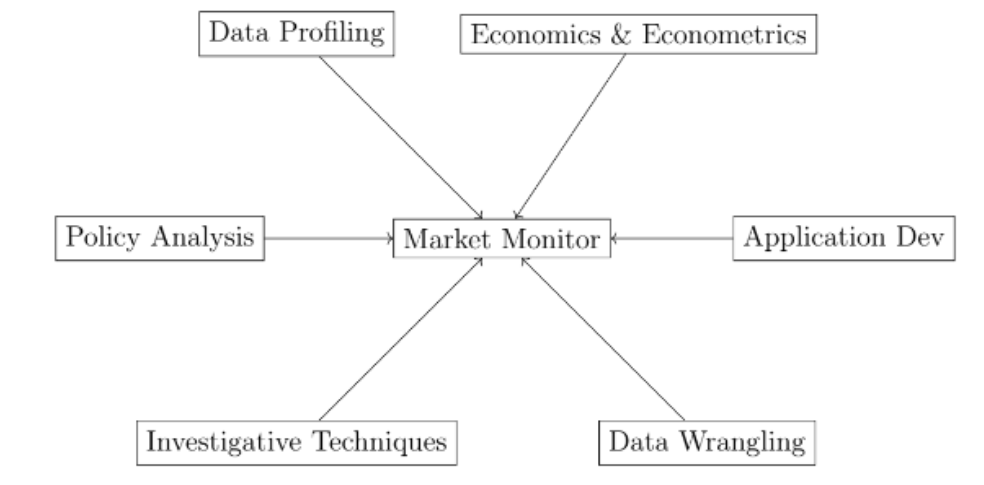
\includegraphics[scale=0.5]{graphic/mkt-monitoring-skill-sets.png}}
\caption{Diverse skill sets of a Market Monitor}
\label{fig:skillset}
\end{figure}

Figure \ref{fig:skillset} illustrates a cross-section of several of the skill sets that market monitoring analysts might possess, based on the researcher's experience of working as a market monitor within Southwest Power Pool's (SPP) MMU. As one may imagine, it can be difficult to find an individual contributor that possesses an all-encompassing understanding of each of these knowledge areas.

\subsection{Landscape of Market Monitoring}

Market monitors have a wide breadth of responsibilities that must be covered by their individual skill sets. Routine market surveillance is a continuous process that must evolve with the behaviors and trading patterns of market participants. As such, market monitors have to observe and investigate market bids and offers made each operating day, analyze generator behavior to identify erratic response to dispatch commands, ensure that participants are not covertly colluding or engaging in price fixing \footnote{Energy market prices are typically set on a marginal, spatial basis (representing the cost of injecting another MW of energy, at a location, in a market territory) \cite{lmpfaq}.}, and ensure that RTOs and ISOs are acting within the rules defined by their FERC-approved Tariff
\footnote{A Tariff is a governing document that outlines the rules for operating (and participating in) an energy market.} documents. 

\subsubsection{Market Monitoring Firms}

The current groups involved with electricity market monitoring (both in North America and internationally\footnote{The US Energy Association (USEA) published a report outlining international, independent market monitoring groups. Many of the international groups on this list come from that report (see References).}) include the following organizations compiled in Table \ref{tab:mmu-roster}. This list is not intended to be exhaustive, as other nations \footnote{See the list of Industry Acronyms for definitions of these regions} in APAC and EMEA may not be reflected here.

\begin{table}[ht]
    \centering
    \begin{tabular}{|p{6cm}|p{5cm}|p{2cm}|}
        \hline
        \textbf{Name of Firm} & \textbf{Market Affiliation} & \textbf{Country} \\
        \hline
        Federal Energy Regulatory Commission (FERC) & Jurisdictional oversight for all US-based energy markets & USA \\
        \hline
        SPP MMU & Southwest Power Pool (Internal) & USA  \\
        \hline
        Potomac Economics & MISO, ERCOT, NYISO, ISO-NE (External) & USA \\
        \hline
        ISO-NE IMM & ISO-NE (Internal) & USA \\
        \hline
        CAISO MMU & California ISO (Internal) & USA \\
        \hline
        Monitoring Analytics & Pennsylvania, New Jersey, Maryland Interconnect (PJM) & USA \\
        \hline
        Market Surveillance Administrator & Alberta & Canada \\
        \hline
        Independent Electricity System Operator (IESO) & Ontario & Canada \\
        \hline
        Canada Energy Regulator & Jurisdictional oversight for all Canadian energy markets & Canada \\
        \hline
        Superintendencia de Electricidad y Combustibles & - & Chile \\
        \hline
        Agencia Nacional de Energia Electricia & - & Brazil \\
        \hline
        Ente Regulador de la Electricidad & - & Argentina \\
        \hline
        Superintendencia de Electricidad & - & Bolivia \\
        \hline
        Regulation on Wholesale Energy Market Integrity and Transparency (REMIT) & European Union Agency for the Cooperation of Energy Regulators & Europe \\
        \hline
        AER & Australian Energy Regulator & Australia \\
        \hline
        NZEA & New Zealand Electricity Authority & New Zealand \\
        \hline
    \end{tabular}
    \caption{A Roster of Groups with Market Monitoring Authority}
    \label{tab:mmu-roster}
\end{table}

\section{Conducting Information Quality Research in Market Monitoring}

The case-study of Enron Corporation sets both a unique and compelling stage for the role that Information Quality and Information Science-based research can play in improving the business impact of an independent market monitor. Included amidst Enron Corporation’s numerous failures of governance is a lack of access and understanding of the complex data generated by the energy industry. The operation of such a large system and marketplace can lead to many siloed data stores, undocumented schemas, and a slew of other IQ-based problems that can also be seen in market monitoring.

Furthermore, the cross-section of skills that market monitors must possess (to effectively perform their job functions) also underscores the importance that data literacy and data quality improvement hold in the market monitoring domain. An architecture solution, proposed as part of the deliverables of this dissertation, is paramount to designing a system to aid market monitoring staff in their work.

\subsection{Subject Matter Expert (SME) Discussions}

The potential use of this dissertation is driven, in part, by the opinions of subject matter experts in the field of electric energy. In support of this research, I have consulted multiple members in different sectors of the industry, including 2 professionals in enterprise asset management, and a separate discussion with a staff member in energy regulation. One such staff member, Dr. Kennedy Oyoo, performed information systems research in a different sector of the energy grid- “power and utilities”- focusing on the distribution of electricity to end users.

Energy utilities struggle with a similar issue to those faced by market monitors- siloed data exists in different systems, and can exist with vastly different data quality scores (in terms of completeness, accuracy, etc.) Dr. Oyoo’s research found that a key step- data validation- was missing from the ETL processes of an energy utility. Part of the research completed in his project resulted in an information template-based prototype system that cleansed and validated utility data according to automated assertion rules. Such a methodology has potential impacts for the market monitoring discipline, and can have an influence on the resulting system architecture of this dissertation (particularly in utilizing a system of templates to fetch market data).
